
%----------------------------------------------------------------------------------------
%	CHAPTER X
%----------------------------------------------------------------------------------------

\chapter{Notação de movimento}


%%%%%%%%%%%%%%%%%%%%%%%%%%%%%%%%%%%%%%%%%%%%%%%%%%%%%%%%%%%%%%%%%%%%%%%%%%%%%%%%
%% SECTION
%%%%%%%%%%%%%%%%%%%%%%%%%%%%%%%%%%%%%%%%%%%%%%%%%%%%%%%%%%%%%%%%%%%%%%%%%%%%%%%%
\section{Posturas e movimentos}

pontos de parada
\begin{itemize}
\item Frente atras (ex: cruzado, abertura lateral).
\item Abertura lateral (ex: balanço, cruzado).
\item Cruzado | X (ex: caminhada, romario).
\item Cruzado invertido (ex: caminhada de casal).
\item Facão (ex: pião).
\item Facão invertido (ex: escovinha).
\end{itemize}


%%%%%%%%%%%%%%%%%%%%%%%%%%%%%%%%%%%%%%%%%%%%%%%%%%%%%%%%%%%%%%%%%%%%%%%%%%%%%%%%
%% SECTION
%%%%%%%%%%%%%%%%%%%%%%%%%%%%%%%%%%%%%%%%%%%%%%%%%%%%%%%%%%%%%%%%%%%%%%%%%%%%%%%%
\section{Valores por defeito na postura do corpo}


\begin{itemize}
\item O abraço do condutor e firme e mantém a mesma distancia no casal.
\item O pé que é movimentado ganha o 100 $\%$ do peso,
\item Leva o peso do corpo por ação do quadril. o quadril arrasta a perna não ao contrario.
\item Mantém o paralelismo de ombros entre o casal.
\item O pé de apoio do condutor aponta sempre para ao seguidor, sempre que seja fisicamente possível.
\end{itemize}


%%%%%%%%%%%%%%%%%%%%%%%%%%%%%%%%%%%%%%%%%%%%%%%%%%%%%%%%%%%%%%%%%%%%%%%%%%%%%%%%
%% SECTION
%%%%%%%%%%%%%%%%%%%%%%%%%%%%%%%%%%%%%%%%%%%%%%%%%%%%%%%%%%%%%%%%%%%%%%%%%%%%%%%%
\section{Símbolos indicadores de tempo e peso do corpo}\index{Símbolos de tempo e peso do corpo}

os símbolos que representam que o pé que executa o movimento é o esquerdo são:
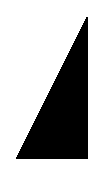
\includegraphics[height=11pt]{chapters/cap-partitura/torso-pe-esquerdo-contratempo.eps},
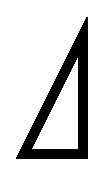
\includegraphics[height=11pt]{chapters/cap-partitura/torso-pe-esquerdo-tempo.eps},
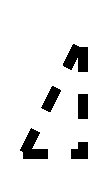
\includegraphics[height=11pt]{chapters/cap-partitura/torso-pe-esquerdo-indef.eps};
por outro lado os símbolos que representam que o pé que executa o movimento é o direito são:
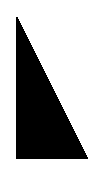
\includegraphics[height=11pt]{chapters/cap-partitura/torso-pe-direito-contratempo.eps},
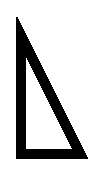
\includegraphics[height=11pt]{chapters/cap-partitura/torso-pe-direito-tempo.eps},
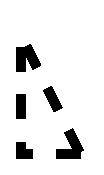
\includegraphics[height=11pt]{chapters/cap-partitura/torso-pe-direito-indef.eps};

\begin{abc}[name=chickchicktum1]
X: 1 % start of header
K: C % scale: C major
M:2/2
T: Chick-Chik Tum
V:1 clef=treble name="Instrumento 1" sname="Inst. 1"
V:2 clef=treble name="Instrumento 2" sname="Inst. 2"
[V:1] "Chik"G4 "Tum"E4 | "Chik"G4 "Tum"E4 |
[V:2] z2"Chik"G2 z4 | z2"Chik"G2 z4 |
\end{abc}

A Tabela \ref{tab:simbolospe}
\begin{table}[!hbt]
\caption{Tempos de espera apos levar o peso do corpo.}
\begin{center}
\begin{tabular}{|l |l | l |}
\hline
Tempo de espera  & Pé esquerdo & Pé direito \\
\hline
\hline
Médio tempo  & 
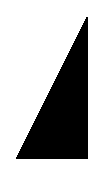
\includegraphics[height=11pt]{chapters/cap-partitura/torso-pe-esquerdo-contratempo.eps}   & 
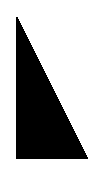
\includegraphics[height=11pt]{chapters/cap-partitura/torso-pe-direito-contratempo.eps}   \\
\hline
Tempo  & 
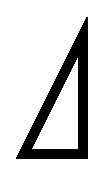
\includegraphics[height=11pt]{chapters/cap-partitura/torso-pe-esquerdo-tempo.eps}   & 
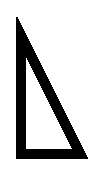
\includegraphics[height=11pt]{chapters/cap-partitura/torso-pe-direito-tempo.eps}   \\
\hline
Indefinido & 
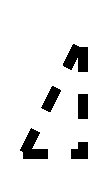
\includegraphics[height=11pt]{chapters/cap-partitura/torso-pe-esquerdo-indef.eps}   & 
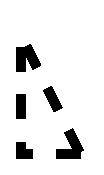
\includegraphics[height=11pt]{chapters/cap-partitura/torso-pe-direito-indef.eps}   \\
\hline
\hline
\end{tabular}
\end{center}
\label{tab:simbolospe}
\end{table}
